\documentclass[preview]{standalone}

\usepackage{amsmath}
\usepackage{amssymb}
\usepackage{stellar}
\usepackage{bettelini}

\hypersetup{
    colorlinks=true,
    linkcolor=black,
    urlcolor=blue,
    pdftitle={Biologia},
    pdfpagemode=FullScreen,
}

\begin{document}

\title{Biologia}
\id{biologia-sintesi-proteine}
\genpage

\begin{snippet}{4376f191-0793-4b43-922f-2894aa107cf4}
    Le informazioni necessarie per costruire sequenze
    differenti di aminoacidi (proteine differenti) sono
    contenute nel DNA.
    
    Per rendere possibile la costruzione delle proteine sono
    necessari altri due tipi di acidi nucleici:
    
    \begin{itemize}
        \item l'RNA messaggero (m-RNA): porta il messaggio del
            gene sul luogo della sintesi proteica (ribosoma).
        \item l'RNA di trasporto (t-RNA): trasporta al ribosoma il
            giusto aminoacido in corrispondenza della sua
            tripletta di codice.
    \end{itemize}
    
    I ribosomi leggono l'm-RNA, i t-RNA (sempre costruiti da filamenti di RNA)
    matchano tre geni alla volta, e se il gene
    viene matchato inseriscono il loro amminoacido nel ribosoma, il quale
    aggiunge al filamento della proteina che si sta creando.
\end{snippet}

\begin{snippet}{protien-synthesis-illustration}
    \begin{center}
    \begin{figure}[th]
        \centering
        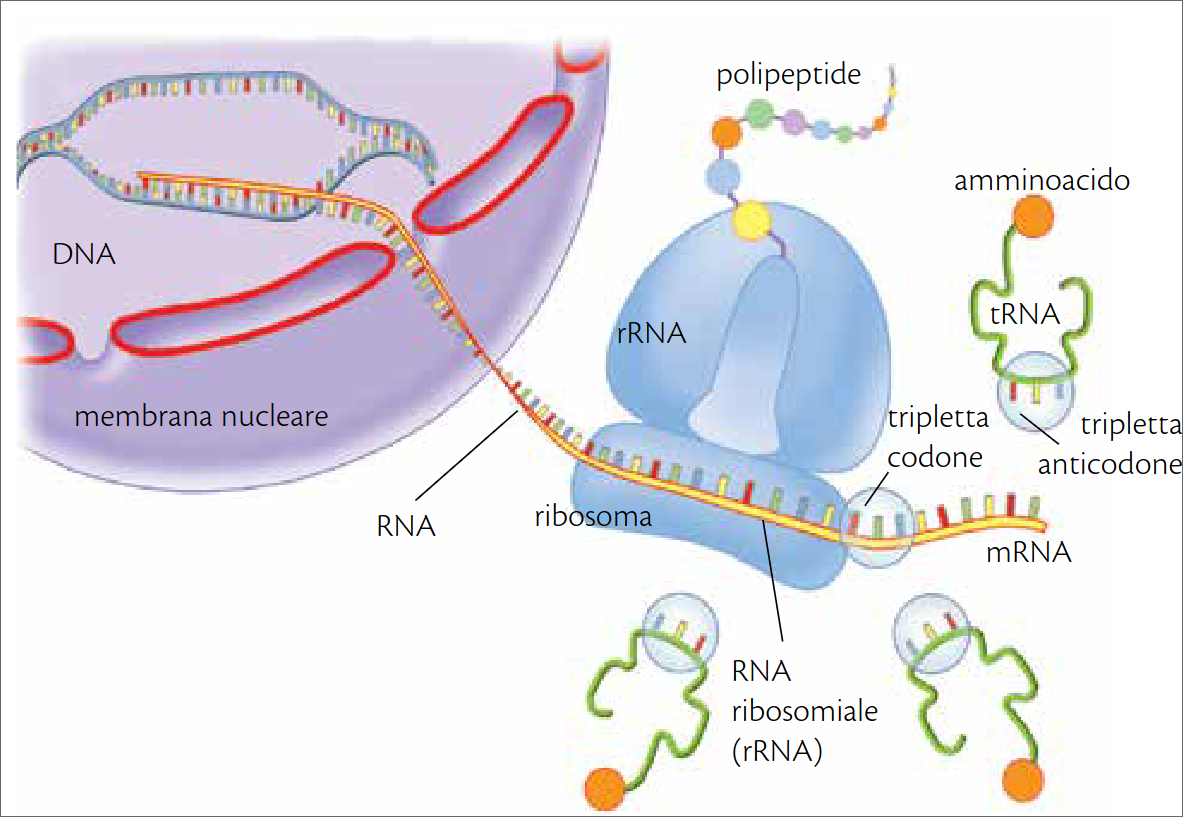
\includegraphics[width=0.75\textwidth]{./resources/protein_synthesis.png}
    \end{figure}
    \end{center}
\end{snippet}

\begin{snippetdefinition}{codice-genetico-definizione}{Codice genetico}
    Il \textit{codice generico} è l'insieme
    delle corrispondenze che mettono in
    relazione le triplette di DNA con gli amminoacidi.
\end{snippetdefinition}

\begin{snippet}{aeb66419-14a7-4757-8393-f098c06553e6}
    Il codice genetico permette di tradurre il codice del DNA
    (4 simboli) nel linguaggio delle proteine (20 simboli).

    % immagine con la griglia 4x4 e il cerchio con tutte le combinazioni

    Per tradurre il DNA in proteina è necessaria una copia intermedia
    (chiamata \textit{mRNA}).
\end{snippet}

\begin{snippetnote}{ebc0922e-7fb0-49c4-8b91-181b6a44b697}{}
    Il DNA \textbf{non} viene copiato, bensì viene
    \textit{trascritto} in mRNA.
\end{snippetnote}

\begin{snippet}{37930bd8-3f4b-4ac9-8ea4-1f5572b0c0ec}
    La tripletta AUG (amminoacido \textit{Met}) è quella di start,
    mentre le combinazioni di stop (UAA, UAG, UGA) si ferma.
    Molteplici triplette diverse codificano il medesimo amminoacido.
\end{snippet}

\end{document}